In this chapter the results from the experiments will be shown and analyzed. First, the model will be discussed without any policies in effect. Following this, the base model is tested for it's performance against multiple scenarios. Finally, the policies are implemented, and their robustness to the earlier scenarios tested. This analysis serves an interpretation of the relative cost-effectiveness of the chosen policies, allowing for comparison of real-world cost of implementation. 

\iffalse
1.	Show and explain results without policies
2.	Show and explain consequences of scenarios for model behaviour
3.	Show and explain consequences of policies for each scenario (i.e., robustness) 
\fi
\subsection{Base Model}

The model was first run without any policies in place to study the effects of the scenarios on the situation as is. Afterwards, it will be run as a part of the scenarios to see how the status quo fares in our defined scenarios. 

The model was run without any scenarios to generate behaviour, dubbed the base run. The behaviour of the KPIs was studied for this base behaviour.

\begin{figure}[h!]
    \centering
    \begin{minipage}{0.45\textwidth}
        \centering
        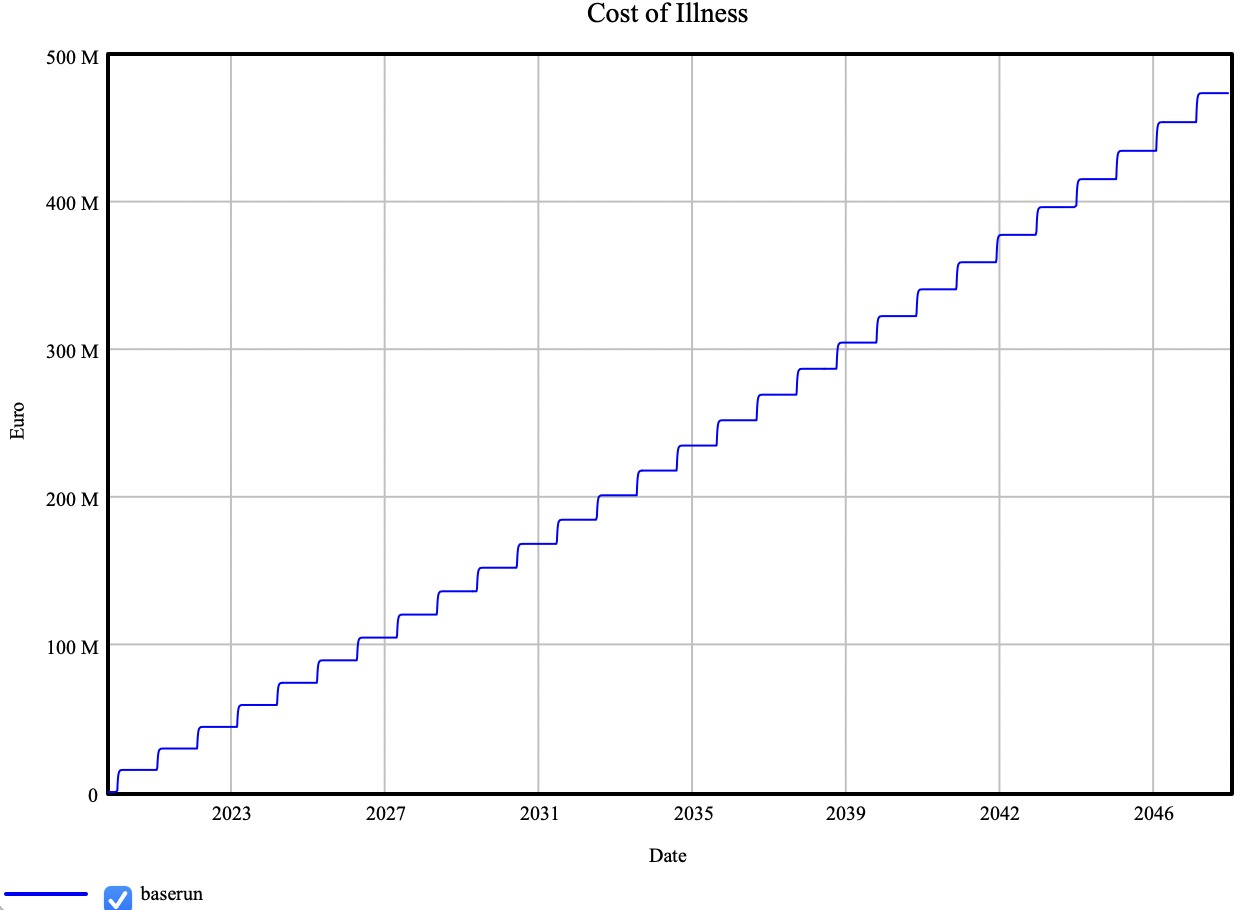
\includegraphics[width=1\textwidth]{images/base_COI.jpeg} % first figure itself
        \caption{Cost of Illness in the base run}
        \label{fig:b_coi}
    \end{minipage}\hfill
    \begin{minipage}{0.45\textwidth}
        \centering
        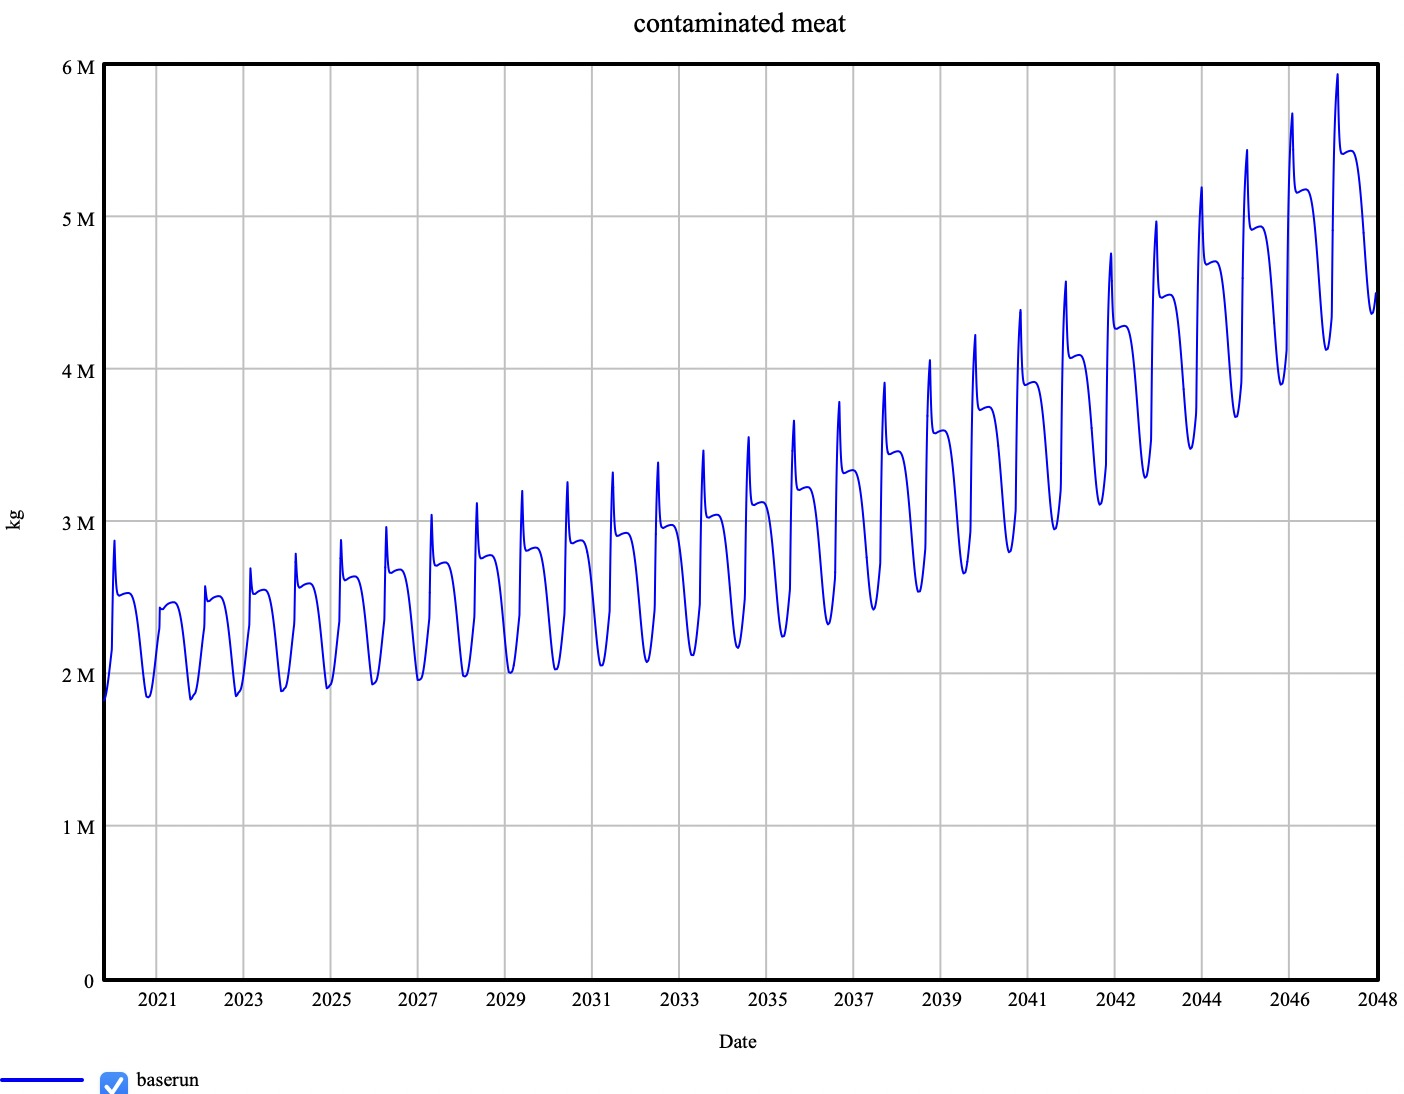
\includegraphics[width=1\textwidth]{images/base_meat.jpeg} % second figure itself
        \caption{Contaminated chicken meat in the base run}
        \label{fig:b_meat}
    \end{minipage}
\end{figure}

\begin{figure}[h!]
    \centering
    \begin{minipage}{0.45\textwidth}
        \centering
        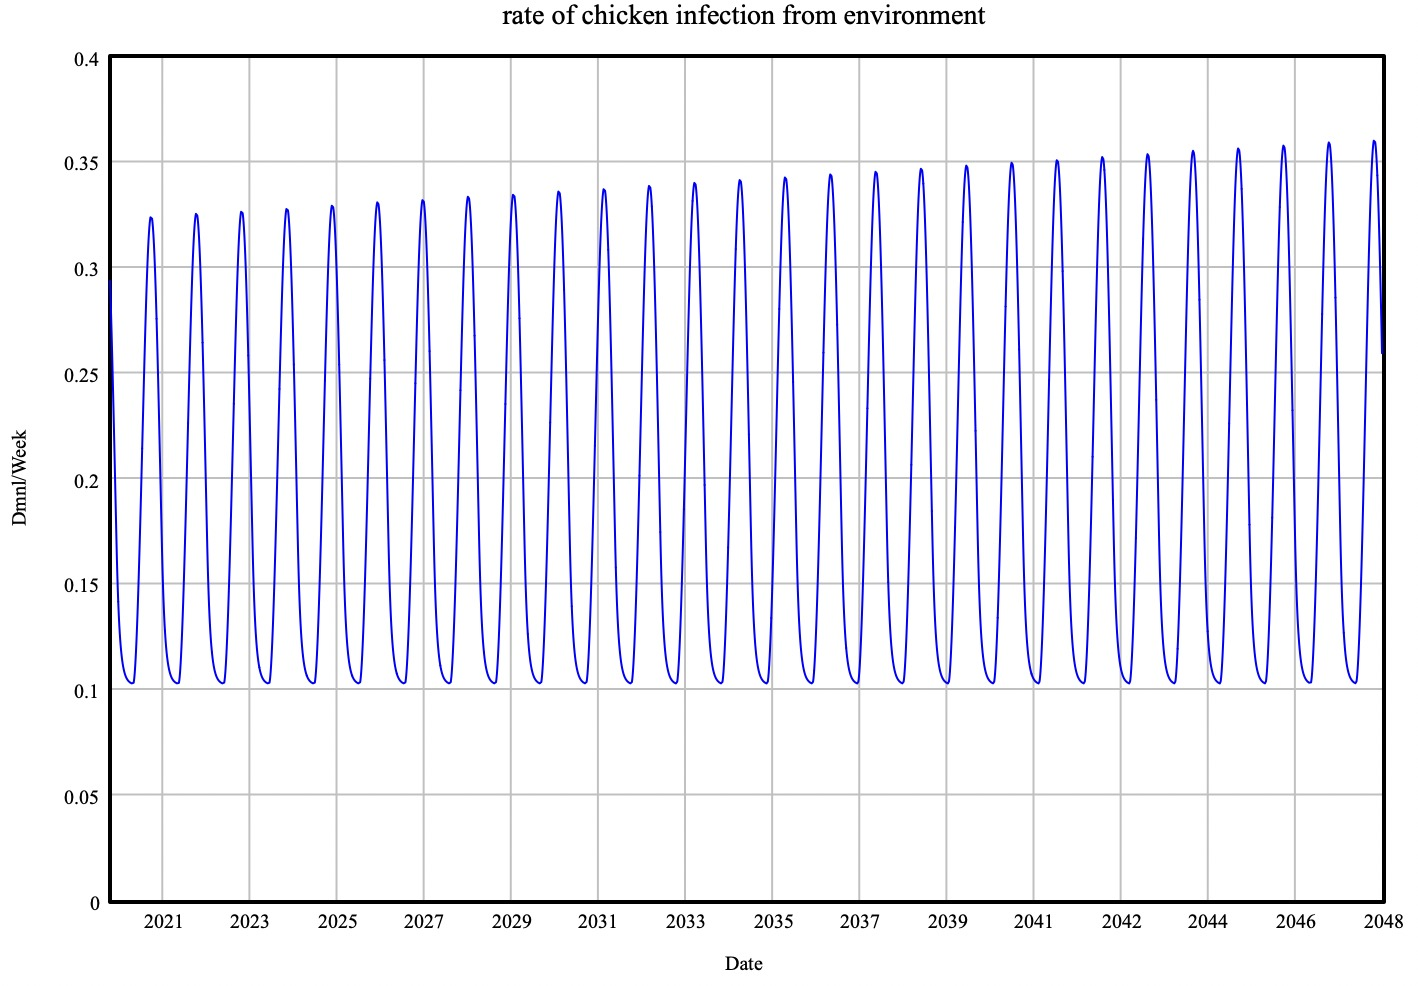
\includegraphics[width=1\textwidth]{images/base_chicken.jpeg} 
        \caption{Chicken infections from environment in the base run}
        \label{fig:b_chicken}
    \end{minipage}\hfill
    \begin{minipage}{0.45\textwidth}
        \centering
        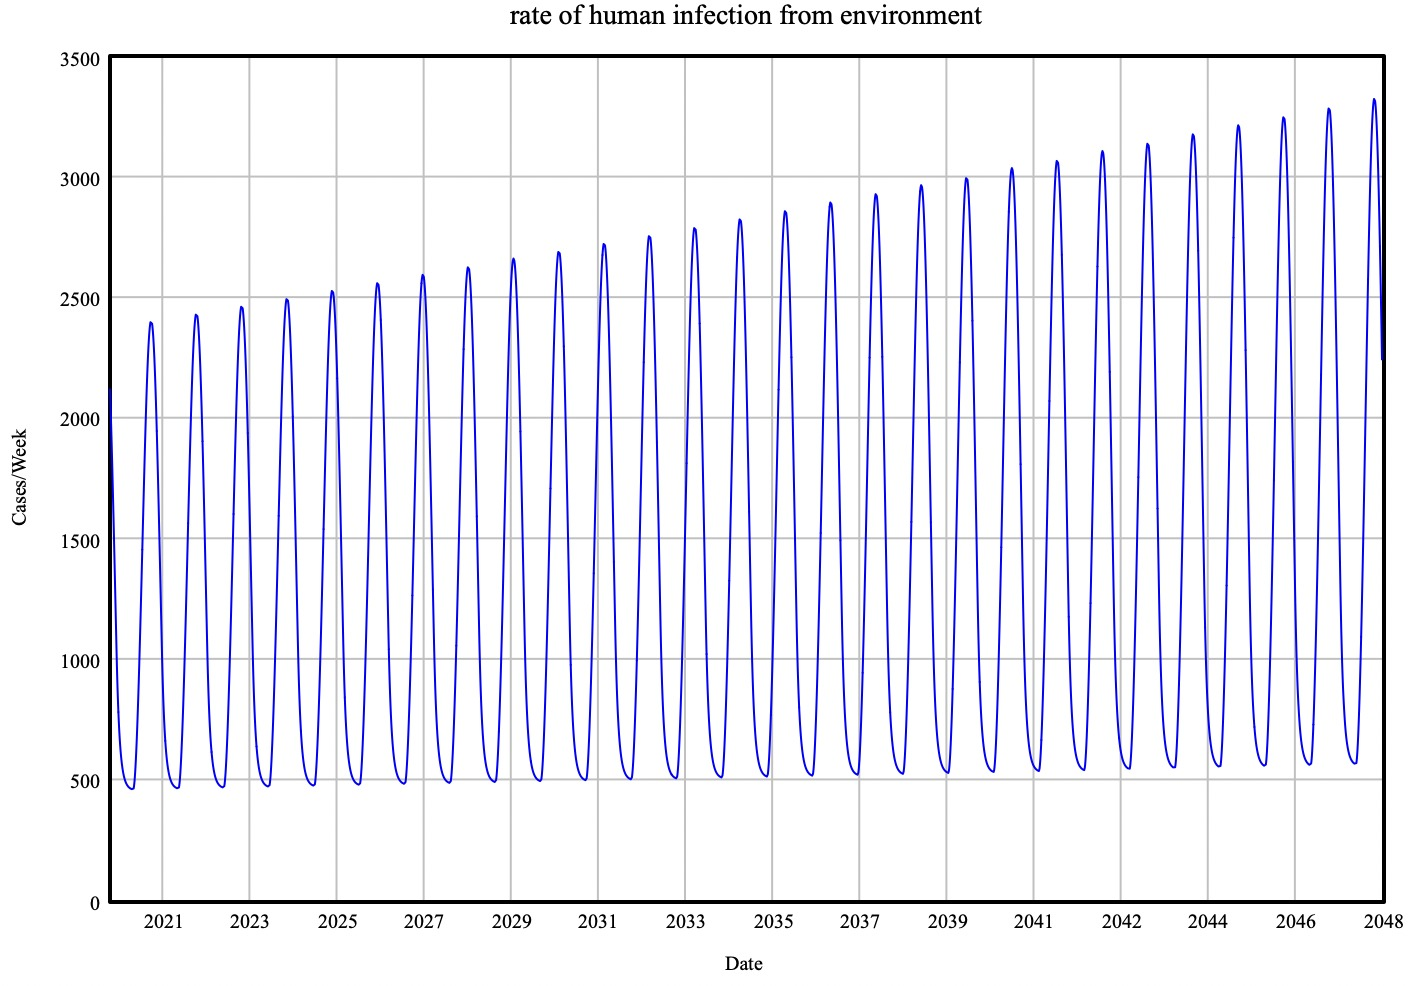
\includegraphics[width=1\textwidth]{images/base_human.jpeg}
        \caption{Human infections from environment in the base run}
        \label{fig:b_human}
    \end{minipage}
\end{figure}

The model generated behaviour that was generally consistent with the dynamic hypothesis, with three main exceptions:

The contaminated meat stock (Figure \ref{fig:b_meat}) exhibits unusual behaviour due to a structural uncertainty linking the number of \textit{campylobacter} cases to changes in meat consumption. After a given threshold number of cases have occurred in the population, we assume there would be a change in behaviour of people choosing to consume less chicken meat to avoid infections, this results in a temporary spike in the contaminated meat stock while the poultry industry responds to changing consumer demand.

Secondly, we did not account for seasonality in the development of the contaminated meat stock. It had been conceptualised in the aggregate sense, leaving the seasonality out of it. 

The model produces a stair-like graph for the cost of illness, where we had hypothesized a straight line instead. This has to with the switch in units mentioned in section \ref{s:verification}, where the model goes from weeks to years. This means that the increase in Cost of Illness occurs once every 52 weeks and then remains the same for the rest of the year, resulting in the stairs we can see in (Figure \ref{fig:b_coi}). Should the time step of the model have been consistent, it would have resulted in a straight line as hypothesized. 

\textcolor{red}{Note on cost of illness: values are indexed to prices in the year 2000. Prices should be adjusted for the year in which the model is being used, based on a suitable inflation metric}

\subsection{Policy Robustness}
% Try and answer these three questions for each policy:
    %1. What scenarios is your policy robust/not robust to?
    %2. Why might this be the case?
    %3. What are the implications for policy implementation?
\subsubsection{Reducing human exposure to flies}
\label{reducing human exposure to flies}



\subsubsection{Pest Control}
\label{sec: pest control}
The Pest Control policy was found to be most robust against climate change scenarios, with no observable difference between KPI outcomes for different climate scenarios. This is because the policy is pegged to temperature, effectively capping propagation of flies at higher temperatures. However, it is less robust to changes in seasonality, wherein after 2030, there is a divergence in outcomes. For scenarios with greater seasonality, the policy of controlling fly populations is less capable of responding to larger variation in temperature.


Predictably, the policy doesn't influence changes in public health scenarios, as the effects are too far downstream of the policy for pest control to have a material impact.

As pest control is robust to climate variation, we recommend that policy-makers consider this as an effective policy under futures with climate uncertainty, but should be paired with other policies to manage for downstream effects (especially with respect to public health scenarios). In the near term, this policy is unlikely to be cost-effective, however, from 2030 onward (assuming climate projections are representative), the economic effects of the policy will be large enough (more than EUR 10 million) to justify expenditure on this policy.

Note: This policy is implemented without delay. It was assumed that if a policy is in place to exterminate flies once temperature exceeds 20 degrees Celsius, government can effectively trigger an immediate extermination at relevant locations.

\subsubsection{Safe Slaughtering}
\label{sec: safe slaughtering}


\subsubsection{Food safety and handling}
\label{sec: food safety}

\subsubsection{Poultry consumption behaviour}
\label{sec: consumption behaviour}
% This is essentially, an extreme values behaviour. It's assumed that the government will not enact this policy except for under extenuating circumstances, whereby case numbers get so high that all other policy options are exhausted, and the government needs to ask citizens to reduce poultry consumption.